\documentclass[a4paper,12pt,openany]{report}
\usepackage[utf8]{inputenc}
\usepackage{amsmath, amssymb}
\usepackage{graphicx}
\usepackage{hyperref}
\usepackage{subcaption}
\graphicspath{ {UML_Flowcharts/} }
\usepackage[dvipsnames]{xcolor}
\usepackage{geometry}
\geometry{tmargin=0.5in}
% Book's title and subtitle
\title{\Huge \textbf{Software Design Document}
 \\
 \Huge \textbf{ Engineering Drawing Software} \vspace{10pt}\\\huge{COP290 Project }}
% Author
\author{\textsc{Arpan Mangal}
 \\
 \textsc{Deepanshu Jindal}}

%\definecolor{indexColor}{rgb}{0.0742, 0.188, 0.2734}
\hypersetup{
  colorlinks   = true, %Colours links instead of ugly boxes
  urlcolor     = blue, %Colour for external hyperlinks
  linkcolor    = black,%brown, %191970, %Colour of internal links
  citecolor   = red %Colour of citations
}

\begin{document}

%\frontmatter
\maketitle

%\tableofcontents
%\listoffigures
%\listoftables

%\mainmatter

\chapter*{Introduction}
This document contains a brief design specification of the Engineering Drawing Software. It mainly specifies how our user will interact with the software and what all functionalities are provided by our software.

Figure 1 provides an overall view of how the user will see the software and various options available.
\begin{figure}[h]
	\centering
	\makebox[\textwidth][c]{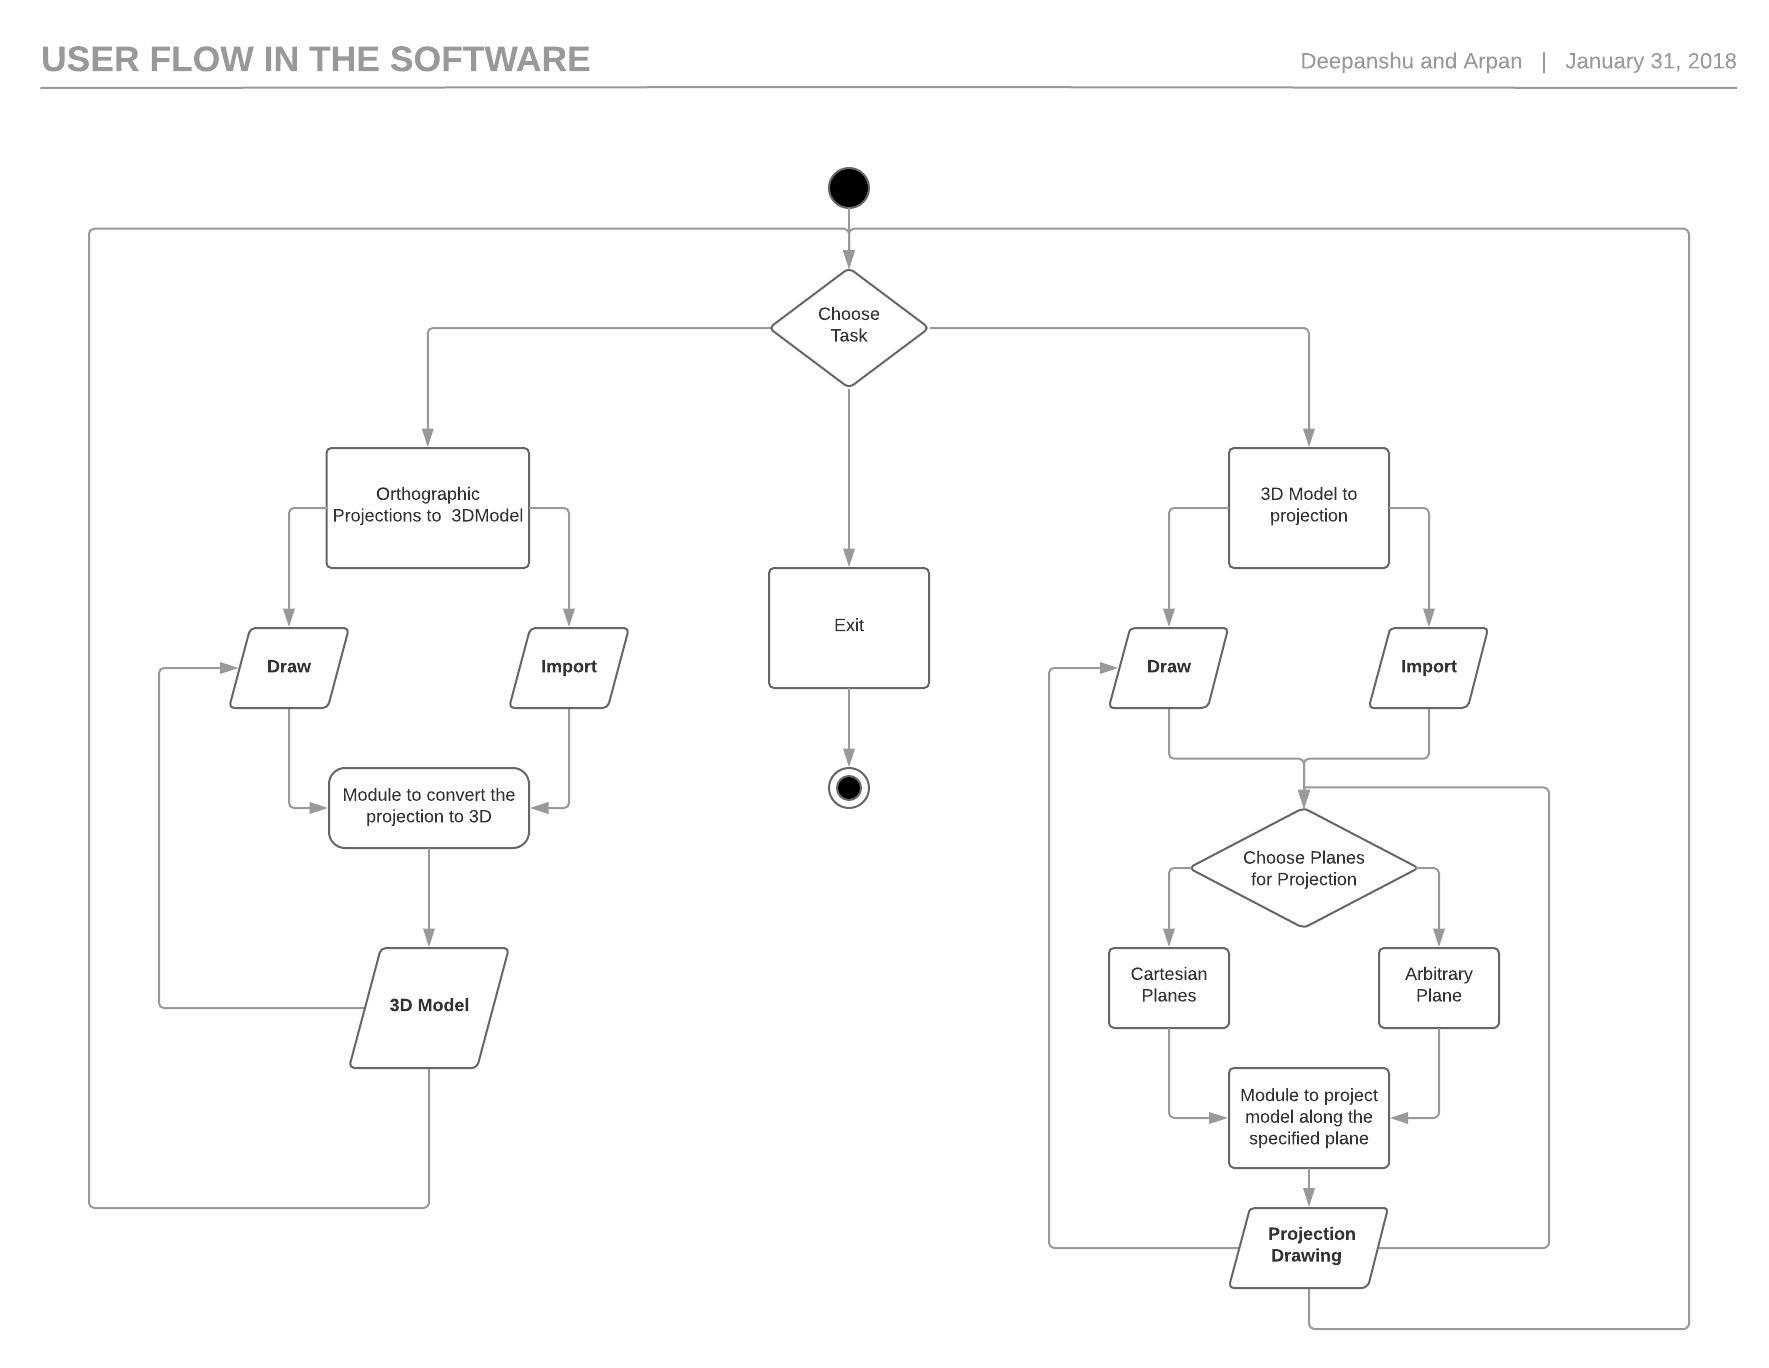
\includegraphics[scale=0.7]{Flow_Diagram}}
	\caption{Use Flow Diagram}
	%\label{a3dObj}
\end{figure}

%On the main menu of the software the user is provided with three options, namely:
%\begin{itemize}
 % \item Orthographic Projections to 3D Model
 % \item 3D Model to Projection
 % \item Exit
%\end{itemize}

\chapter*{3D Model to Projection}
In this option the user has to provide the software with the 3-Dimensional model fo the object for which he wishes to take projections. He is given two choices for providing the object:
\begin{itemize}
  \item Import from an external file
  \item Draw the object and save to a file
\end{itemize}

After providing the 3D object he will be asked to choose the planes on which he wants to take a projection. He can either opt for making the orthographic views of the object or specify any arbitary plane on which to take the projections.\\

After the user provides the required object and specifies appropriate planes the software will proceed to take the projections of the object on the specified planes, the details of which are shown in Fig. 2.\\


This module consists of a central controller which controls how the execution occurs. It first sends the 3D object to the 'Rotate' module to rotate it appropriately in order to project it to the plane specified. After than it commands the projection module to output the projection of the 3D object after giving it the appropriate plane of projection. In case the user had specified an arbitary plane this output also serves as the final output, and in the case that the user had chosen for the three orthographic projections the controller will repeat this process for the three coordinate planes to obtain the three orthographic views which serve as the final output of this module. 

\begin{figure}[h]
	\centering
	\makebox[\textwidth][c]{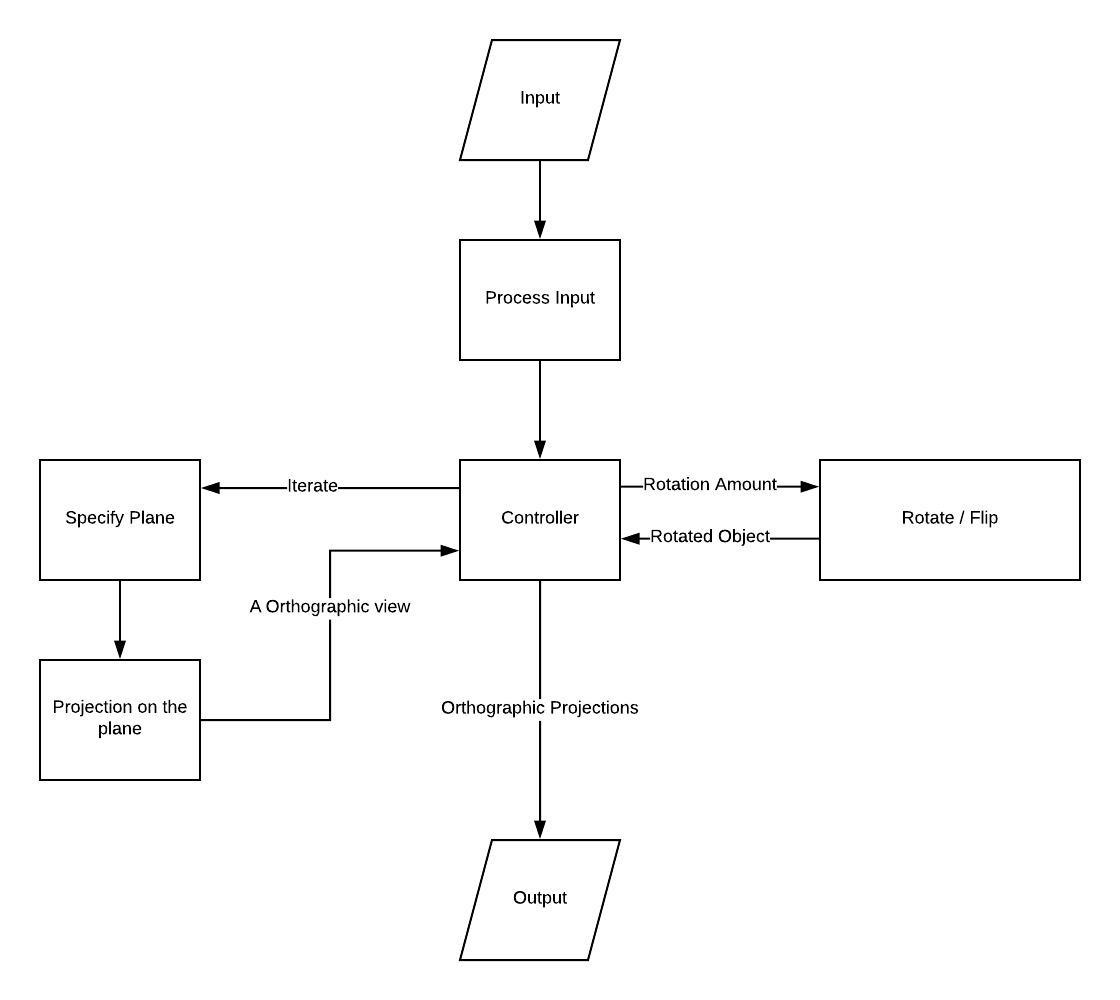
\includegraphics[scale=0.9]{3D_to_2D_Orthographic_Projections}}
	\caption{Projection of the 3D Object along the specified plane}
	%\label{a3dObj}
\end{figure}

\chapter*{Orthographic Projections to 3D Model}
In this option the user has to provide the software with orthographic projections of the 3D object which he wishes to re-construct. He is required to give a minimum of 2 projections for the 3D re-construction. He is also required to specify the point wise correspondence in the three views. He is given two choices for providing the projections:
\begin{itemize}
  \item Import from an external file
  \item Draw the projections and save to a file
\end{itemize}

After the user provides the required projections the software will proceed to convert the projections to 3D, the details of which are shown in Fig. 3.
\begin{figure}[h]
	\centering
	\makebox[\textwidth][c]{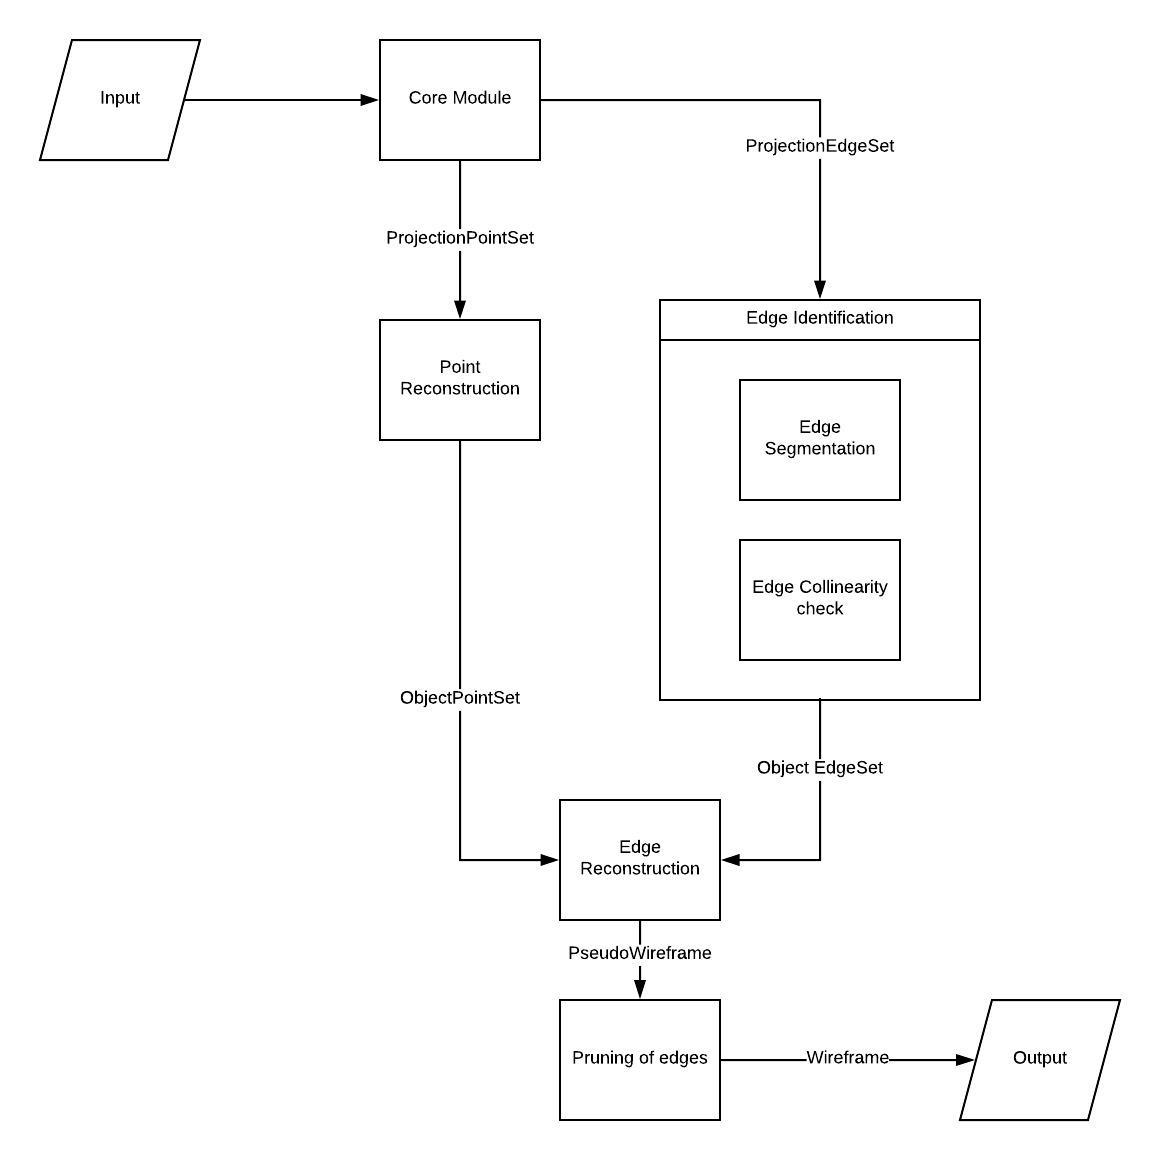
\includegraphics[scale=0.8]{2D_to_3D_Reconstruction}}
	\caption{Orthographic Projections to 3D Re-Construction}
	%\label{a3dObj}
\end{figure}

The software proceeds by first reconstructing the points in 3-Dimensional space. Parellely the software computes extra edges using the Edge Segmentation and Edge Collinearity Algorithms as discussed in the mathematical model. Once it has constructed the point set and the edge set it proceeds with Edge Reconstruction in 3D. The Edge Reconstruction gives a pseudo wire frame model of the actual object. Applying the pruning of edges to the pseudo wire frame gives the actual wireframe of the object which serves as the output of this module.

\chapter*{Draw Module}
As a part of the drawing feature which the software provides the user will be given the functionalities as shown in Fig. 4.
\begin{figure}[h]
	\centering
	\makebox[\textwidth][c]{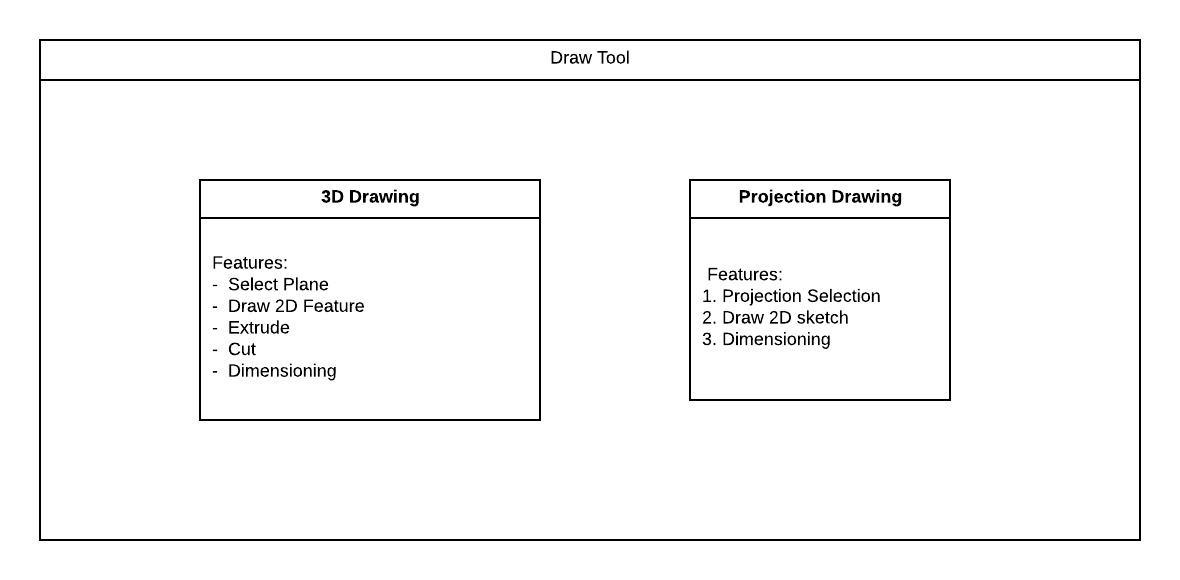
\includegraphics[scale=0.8]{Draw_Module}}
	\caption{Draw Module}
	%\label{a3dObj}
\end{figure}

\end{document}



% \documentclass{report}
%   \usepackage{fullpage}
%   \renewcommand{\baselinestretch}{2}
%   \author{Your Name Here}
%   \title{Your Title Here}
%   \begin{document}
%   \maketitle
%   \tableofcontents

%   \section{Your Section title Here}
%   \subsection{Your Subsection title here}
%   \subsubsection{Your subsubsection title here}
%   \paragraph{Your paragraph title here}
% \end{document}